\documentclass[12pt,oneside]{mwbk}

% ustawienia kodowania pliku i języka
\usepackage[T1]{polski}
\usepackage[utf8]{inputenc}

\usepackage{indentfirst}
\usepackage{graphicx}

%\numberwithin{figure}{section}  % numerowanie obrazków, prefiksowane numerem sekcji
%\numberwithin{table}{section}   % numerowanie tabel, prefiksowane numerem sekcji

% czcionka Times
\usepackage{times}

% odstępy na 1.5 (pomimo, iż linespread jest na 1.3
\linespread{1.3}

% dzielenie wyrazów – większe odstępy, mniej dzielenia
\hyphenpenalty=5000
\tolerance=5000

%import z pliku csv
\usepackage{csvsimple}

%strona tytułowa
\renewcommand {\maketitle}{
\begin {titlepage}
\begin {center}
	\LARGE
	\textbf {PROJEKTOWANIE ALGORYTMOW I METODY SZTUCZNEJ INTELIGENCJI}
	\newline
	\newline
	\textit {SPRAWOZDANIE Z  LABORATORIUM}
	\textbf{ Algorytmy sortujace}
	\newline
	\begin{table}
	\begin{center}
	\begin{tabular}{rl}
	IMIĘ I NAZWISKO & Mariusz Dajczak \\
	NR INDEKSU & 200403 \\	
	TERMIN & czwartek 10:00-12:35 \\
	DATA  & 20.03.2014 \\
	\end{tabular}

	\end{center}
	\end{table}
\end {center}
\end {titlepage}}

\renewcommand*\thesection{\arabic{section}} % zmiana numeracji sekcji 0.X -> X
\begin{document}
\maketitle
\section{Wstęp}
	\indent Sortowanie jest jednym z podstawowych problemów informatyki. Polega na uporzadkowaniu danego zbioru względem 			pewnych cech, np. posortowanie liczb od najmniejszej do najwiekszej. Istnieje wiele algorytmów sortowania. Począwszy od 			prymitywnego sortowania głupiego, poprzez liniowe, bąbelkowe, aż do algorytmów typu Quicksort lub mergesort. Cecha 			wyznaczającą efektywność algorytmu sortowania jest złożoność czasowa. \\
	
\section {Cel ćwczenia}
	\indent Celem ćwiczenia jest zbadanie złożoności obliczeniowej algorytmów sortowania. W sprawozdaniu będę omawiał trzy 			algorytmy:\\
	\indent-sortowanie szybkie\\
	\indent-sortowanie przez scalanie\\
	\indent-sortowanie przez kopcowanie,\\
	Wszystkie te algorytmy mają złożoność czasową nlogn i uważane są za jedne z najszybszych. 
\section {Quicksort}
	\begin{figure}[h]
	\centering
	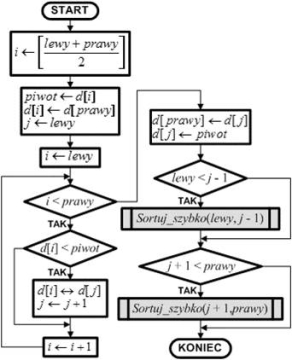
\includegraphics[scale=0.3]{rys/quick.jpg}
	\caption{Schemat blokowy quicksort}
	\end{figure}

	\indent Algorytm sortowania szybkiego jest uważany za najszybszy jesli chodzi o dane losowe. Polega on na metodzie dziel i 			zwyciężaj. Polega to na tym, że zbiór danych zostaje podzielony na dwa podzbiory i każdy z nich jest sortowany niezależnie.
	W średnim przypadku jego złożoność obliczeniowa wynosi $nlogn$ , natomiast w najgorszym $n^{2}$.\\
	\\
	\textbf{Dane pomiarowe}
	\begin{table}[!h]
	\centering
	\begin{tabular}{| l | l | l |}
	\hline
	Rozmiar & Powtórzenia & Czas         \\ \hline
	10      & 20          & 79.3         \\ \hline
	100     & 20          & 1738.25      \\ \hline
	1000    & 20          & 15227.4      \\ \hline
	10000   & 20          & 120922       \\ \hline
	\end{tabular}
	\caption{Pomiary czasu dla Quicksort}
	\end{table}


\section {Merge}
	\begin{figure}[!h]
	\centering
	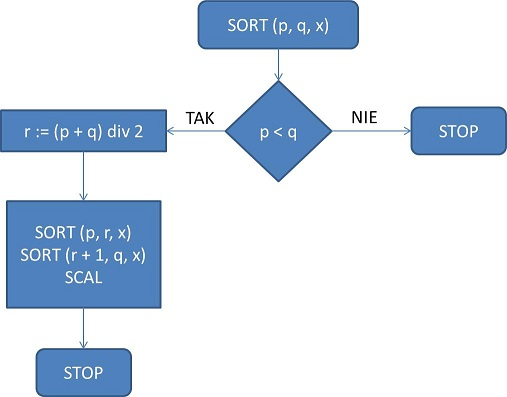
\includegraphics[scale=0.5]{rys/merge.jpg}
	\caption{Schemat blokowy sortowania przez scalanie}
	\end{figure}

	\indent Algorytm sortowania przez scalanie polega na podzieleniu zbioru na jednoelementowe podzbiory, a nastepnie na łaczeniu tych podzbiorów w wiekszy zbiór posortowany. \\
	\\
	\textbf{Dane pomiarowe}
	\begin{table}[!h]
	\centering
	\begin{tabular}{| l | l | l |}
	\hline
	Rozmiar & Powtórzenia & Czas         \\ \hline
	10&5&541\\ \hline
	100&5&5155.4\\ \hline
	1000&5&76662.4\\ \hline
	10000&5&1.37028e+006\\ \hline
	\end{tabular}
	\caption{Pomiary czasu dla Mergesort}
	\end{table}

	
\section {Heapsort}

	\indent Algorytm sortowania poprzez kopcowanie jest najwolniejszym z algorytmów o złożoności $ nlogn $. Polega na stworzeniu kopca binarnego z danych. Nastepnie wartość znajdująca się w korzeniu wedruje na początek tablicy wynikowej, a ostatni element kopca przechodzi do korzenia. Kopiec jest porządkowany i operacja się powtarza, aż do kompletnego rozebrania kopca.\\
	\\
	\textbf{Dane pomiarowe}
	
	
	\begin{table}[h]
	\centering
	\begin{tabular}{| l | l | l |}
	\hline
	Rozmiar & Powtórzenia & Czas        \\ \hline
	10&10&3417.3\\ \hline
	100&10&12390.9\\ \hline
	1000&10&132030\\ \hline
	10000&10&2,58E+06\\ \hline
	\end{tabular}
	\caption{Pomiary czasu dla Heapsort}
	\end{table}

	
\section{Zestawienie}

	\begin{figure}[!h]
	\centering
	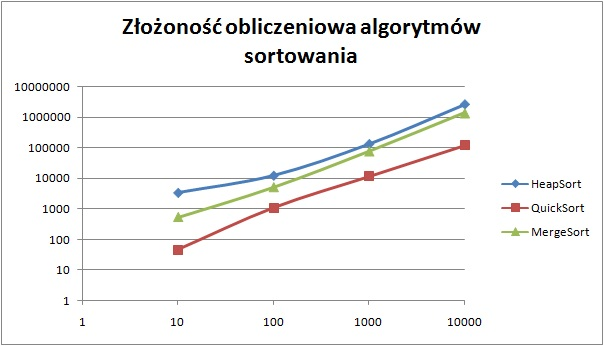
\includegraphics[scale=0.6]{rys/zlozonosc.jpg}
	\caption{Złożoność obliczeniowa algorytmów sortowania}
	\end{figure}

\section{Wnioski}
\indent Wszystkie algorytmy, które testowałem mają złożoność obliczeniową $nlogn$. Najszybszym jest QuickSort, wraz z wzrostem problemu jego przewaga rośnie. MergeSort oraz HeapSort mają zbliżoną charakterystykę złożoności czasowej. 
\indent QuickSort Jest również lepszy pod względem zapotrzebowania na pamięć. Działa on na oryginalnej tablicy z danymi, co powoduje, że praktycznie nie zużywa dodatkowych zasobów. Natomiast pozostałe dwa algorytmy tworzą tablice pomocnicze, co zwieksza złożoność pamięciową.
	
\end{document}